\section{Control and Simulation}
\label{sc:simulation}

Having defined the complete kinematic model via the DH parameters, derived the IK solver, and designed a $C^2$
continuous gait trajectory, we proceed to validate the entire system by simulation. To verify that these
theoretical components function correctly in unison, a digital model of the leg is implemented in the
Simulink \cite{matlab} environment. This simulation serves as a crucial proof-of-concept, allowing for the
verification of the control logic and the workspace before committing to physical hardware. This section details
the open-loop control architecture used for this validation and the construction of the simulation model itself.


\subsection{Open Loop Control Strategy}

The control strategy adopts an open-loop architecture (Figure \ref{fig:control_chain}), deliberately neglecting
external disturbances or modeling errors; its sole purpose is to validate the correctness of the kinematic chain.

It consists in:

\begin{itemize}
  \item \textbf{Path Planning:} The Gait Trajectory Generator outputs the desired Cartesian position $p_d(t)$
    at each time step, given a desired walking speed $v$ and direction $\psi$.
  \item \textbf{Inverse Kinematics:} The desired path $p_d(t)$ is fed into the IK solver, which
    calculates the required vector of joint angles $q_d(t) = [q_1, q_2, q_3]^T$ needed to achieve
    that end-effector position.
  \item \textbf{Leg Model (Plant):} The desired angles $q_d(t)$ are sent as commands to the
    digital twin of the leg, modeled with the aid of the Simscape library.
  \item \textbf{Forward Kinematics:} For validation, the actual joint angles from the simulation model are
    fed into the FK block (based on the DH Table \ref{tab:dh_parameters}). This calculates the resulting
    end-effector position, $p_{sim}(t)$.
\end{itemize}

\begin{figure}[htbp]
    \centering
    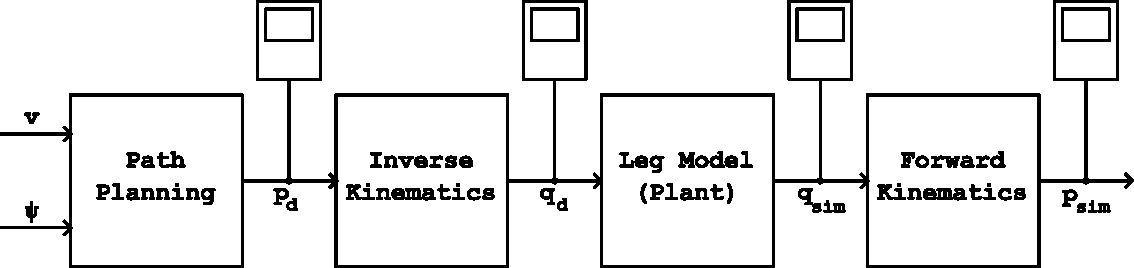
\includegraphics[width=0.98\textwidth]{images/open_loop.pdf}
    \caption{Block Diagram of the Open Loop Control Chain.}
    \label{fig:control_chain}
\end{figure}

A key assumption at this stage is the use of ideal actuators. The joints in the simulation are modeled as
ideal position controllers. This means that when a joint is commanded to go to an angle $q_i$, it achieves
this setpoint almost instantaneously and without error. We are intentionally neglecting the dynamics of the
motors (e.g. torque limits, friction, PID control, and settling time) to isolate the validation purely to the
kinematic model.

The goal is to answer the question: "If the joints go to the angles we calculated, does the foot go to the
position we intended?" The simulation is considered successful if the error between the desired path and the
actual path is approximately close to zero for the entire duration.


\subsection{Digital Simulation}

To create a realistic and physically-grounded representation of the leg, the digital twin is constructed using
Simscape Multibody \cite{simscape}. This MATLAB/Simulink toolbox allows for the modeling of 3D mechanical systems
by defining rigid bodies, joints, constraints, and their spatial relationships.

The leg model (reported in Figure \ref{fig:simscape_model}) is built by importing the CAD (Computer-Aided Design)
files for each link (Coxa, Femur, and Tibia) for a better graphical representation. These rigid bodies are then
connected using 'Revolute Joint' and 'Transformation' blocks at the appropriate locations, corresponding to the
physical actuators and established DH parameters. The joint axes and link-to-link coordinate frames are meticulously
aligned ensuring the simulation model is a one-to-one representation of the theoretical kinematic chain.

\begin{figure}[htbp]
    \centering
    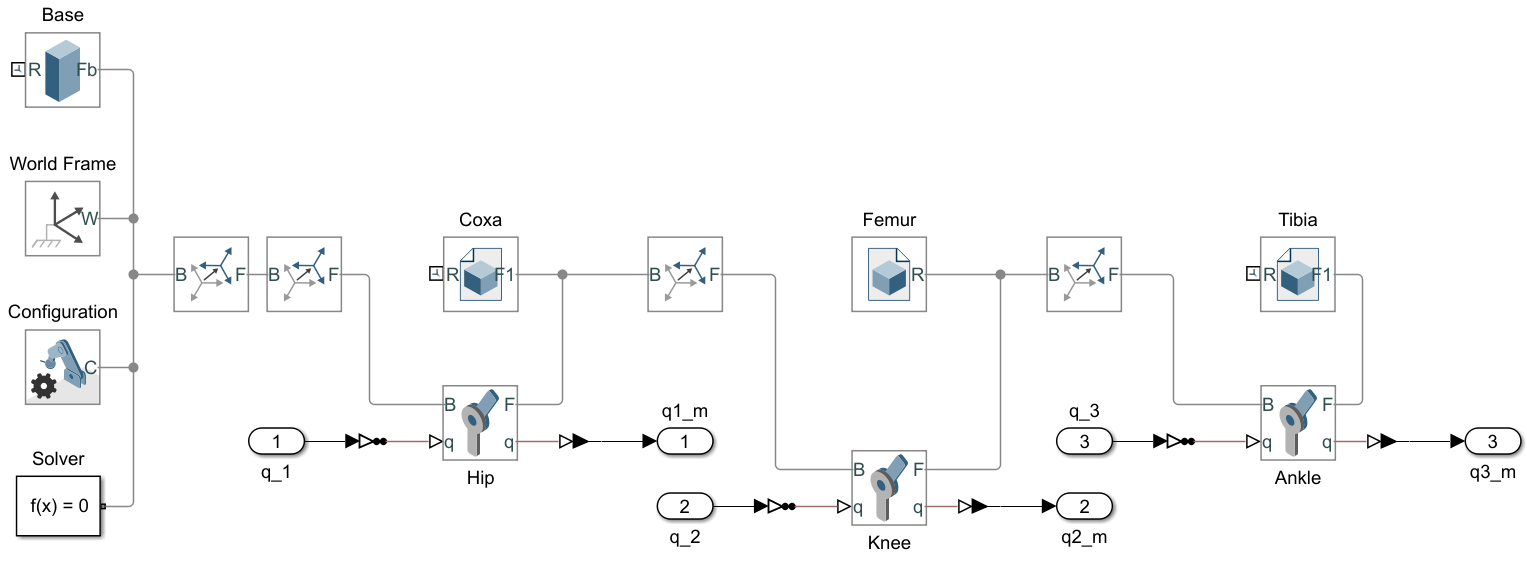
\includegraphics[width=0.98\textwidth]{images/simscape.PNG}
    \caption{Simscape Multibody Limb Model (Plant Block).}
    \label{fig:simscape_model}
\end{figure}

This model serves as the 'Plant' block in the control diagram. The inputs to the model are the three desired
joint angles $q_d(t)$ from the IK block, which drive the 'Sensing and Motion' input of the Revolute
Joint blocks. The outputs are the resulting joint angles and poses, which are passed to the FK validation block
and used to generate the 3D animation (as seen in Figure \ref{fig:rendering_side}) for visual confirmation
of the gait.

\begin{figure}[htbp]
    \centering
    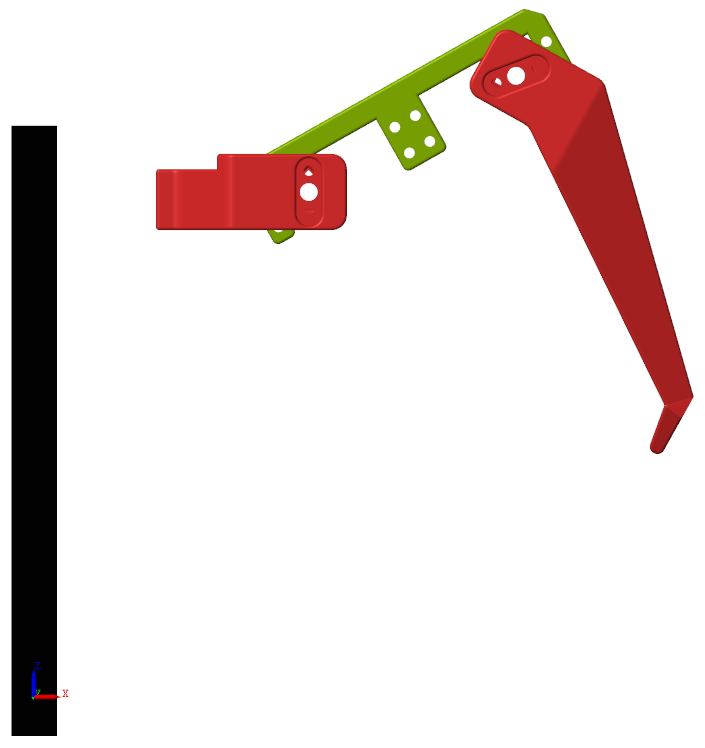
\includegraphics[width=0.48\textwidth]{images/model_side.PNG}
    \caption{3D Rendering of the Simscape Simulation (Side View).}
    \label{fig:rendering_side}
\end{figure}

For the purpose of the digital simulation, the walking direction will be set to be coincident with the y axis
($\vec{\psi} = \vec{y}$).


\subsection{Simulation Results}
\label{sec:simulation_results}

The primary validation of the theoretical model comes from a comparison of the desired Cartesian path (the output
of the Path Generator, $p_d$) against the actual path achieved by the Simscape model (the output of the Forward
Kinematics block, $p_{sim}$). These two trajectories (Figure \ref{fig:gait_z_psi}) are undistinguishable,
confirming the entire kinematic chain — from the DH parameters and IK solver to the FK validation — is
mathematically correct and consistent.

\begin{figure}[htbp]
    \centering
    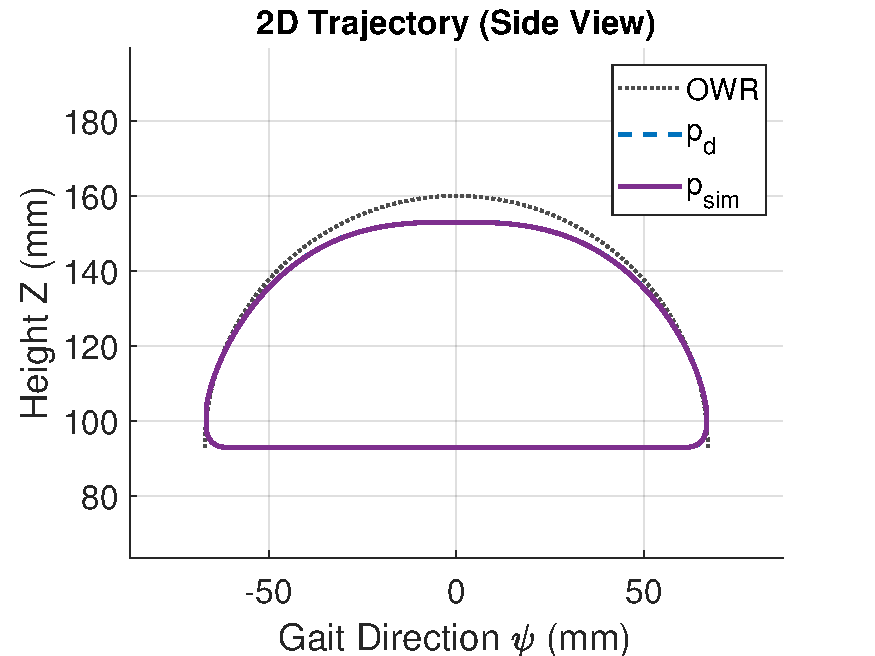
\includegraphics[width=0.65\textwidth]{images/gait_z_psi.pdf}
    \caption{Simulated Gait Ttrajectory in the $Z\psi$-plane (Side View).}
    \label{fig:gait_z_psi}
\end{figure}

The path clearly shows the linear stance phase (where Z is constant) and the smooth, $C^2$ continuous swing
phase, which lifts the foot to the required clearance height. Furthermore, the entire trajectory operates
correctly within the boundaries of the predefined Optimal Workspace Region (OWR).


\subsubsection{Cartesian Space Analysis}

A comprehensive overview of the system's performance in Cartesian space is depicted in Figure \ref{fig:cartesian_results}.

The three plots (X, Y, Z) demonstrate a perfect tracking of the commanded trajectory ($p_d$) as expected from the
ideal actuator assumption. The negligible errors ($e_{sim} \le 0.8\,mm$) are attributed to inertial effects
and a small tracking delay, both reasonable assumptions in real world systems.

\begin{figure}[htbp]
    \centering
    \begin{subfigure}[b]{0.8\textwidth}
        \centering
        
\includegraphics[width=\textwidth]{images/cartesian_trajectories.pdf}
        \caption{Trajectory Tracking}
    \end{subfigure}

    \begin{subfigure}[b]{0.8\textwidth}
        \centering
        
\includegraphics[width=\textwidth]{images/cartesian_errors.pdf}
        \caption{Tracking Errors}
    \end{subfigure}
    \caption{Cartesian-Space Simulation Results.}
    \label{fig:cartesian_results}
\end{figure}


\subsubsection{Joint Space Analysis}

Figure \ref{fig:joint_results} confirms that the Cartesian trajectory is correctly translated into smooth,
continuous joint commands, free of any "snaps" or sudden changes even at phase transition points.

Furthermore, all three trajectories operate comfortably within the designated joint limits, confirming the IK
solver is capable of finding a valid and safe solution.

\begin{figure}[htbp]
    \centering
    \begin{subfigure}[b]{0.8\textwidth}
        \centering
        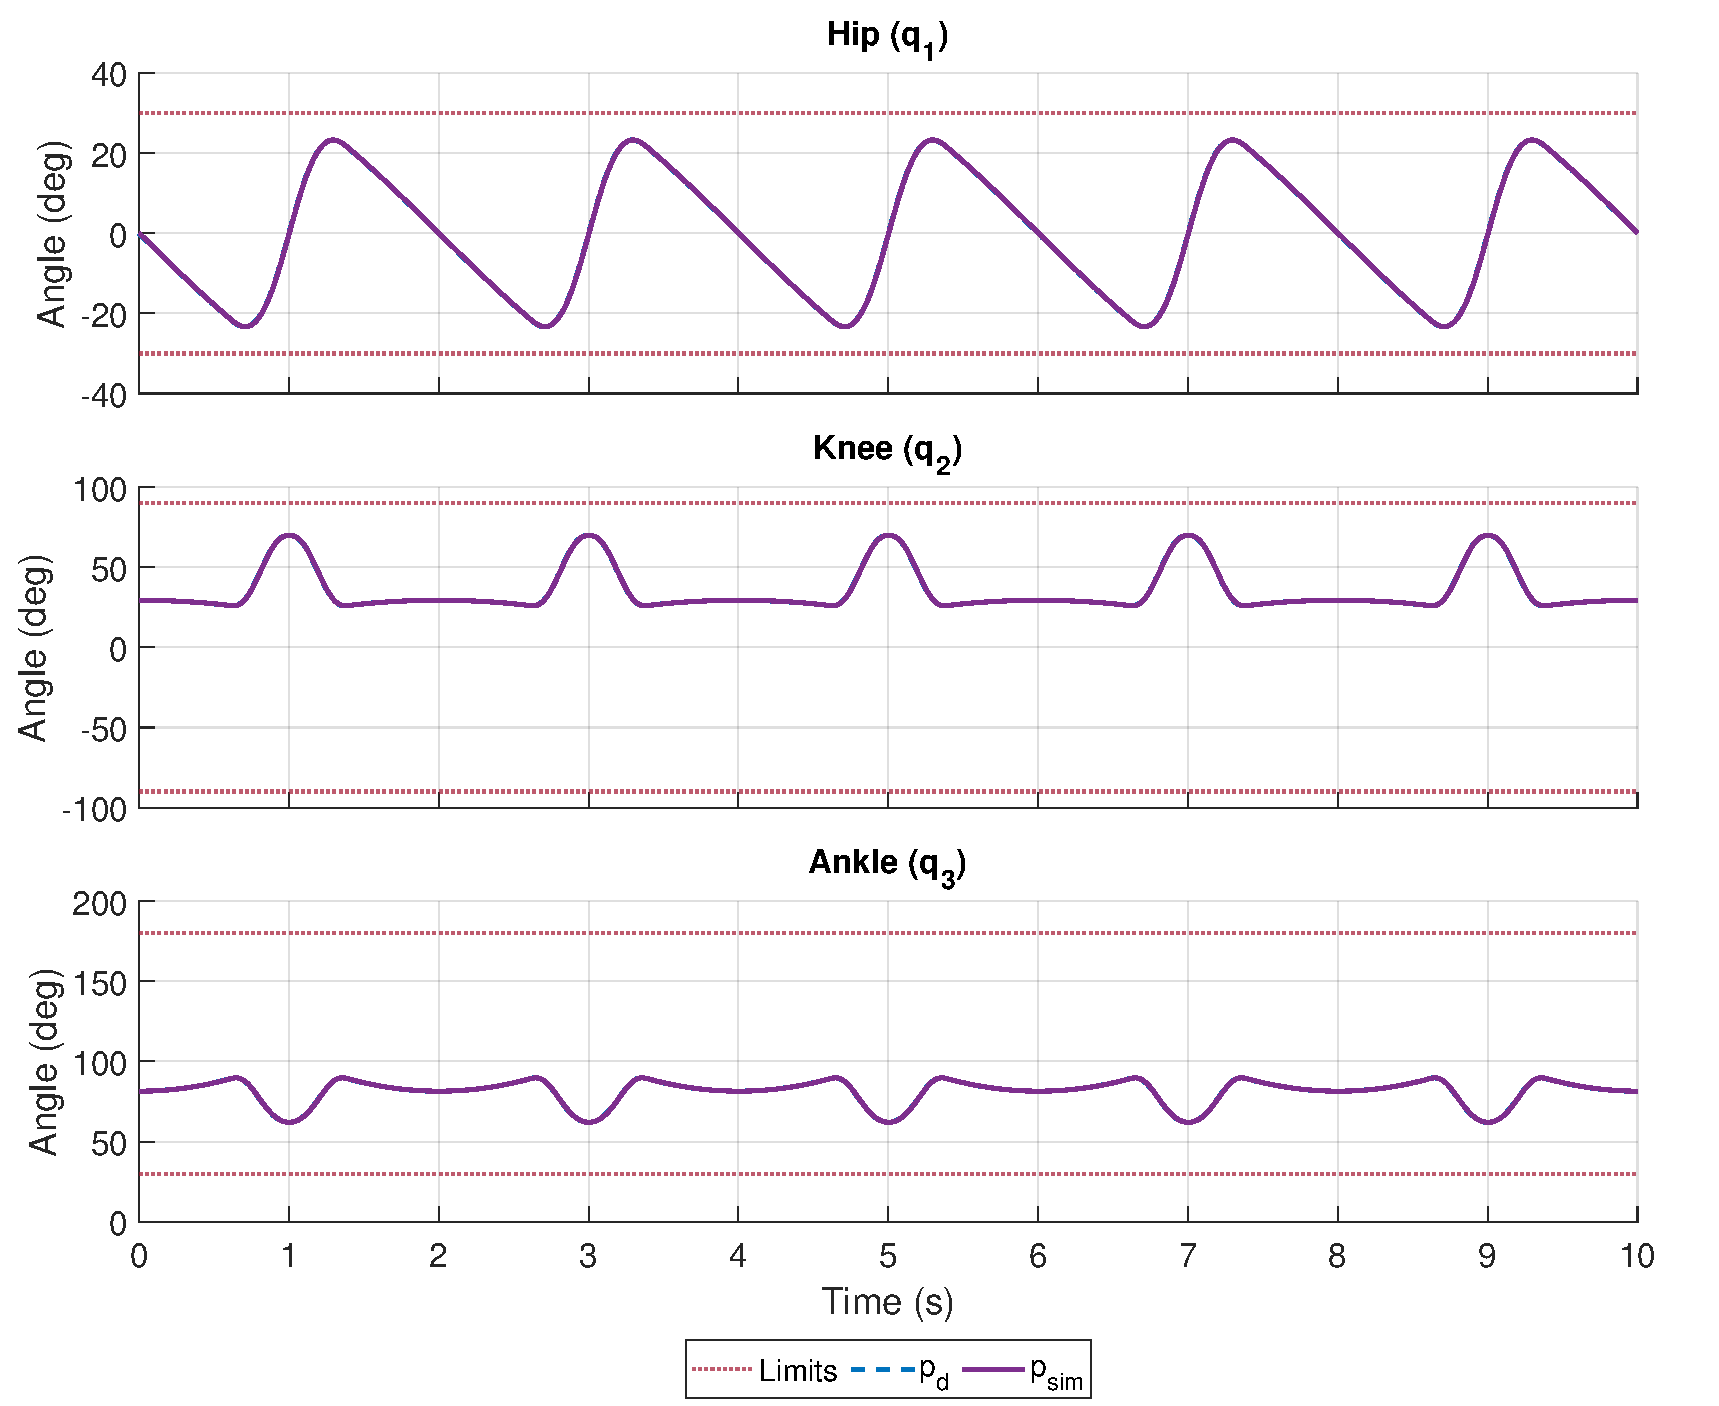
\includegraphics[width=\textwidth]{images/joint_trajectories.pdf}
        \caption{Trajectory Tracking}
    \end{subfigure}

    \begin{subfigure}[b]{0.8\textwidth}
        \centering
        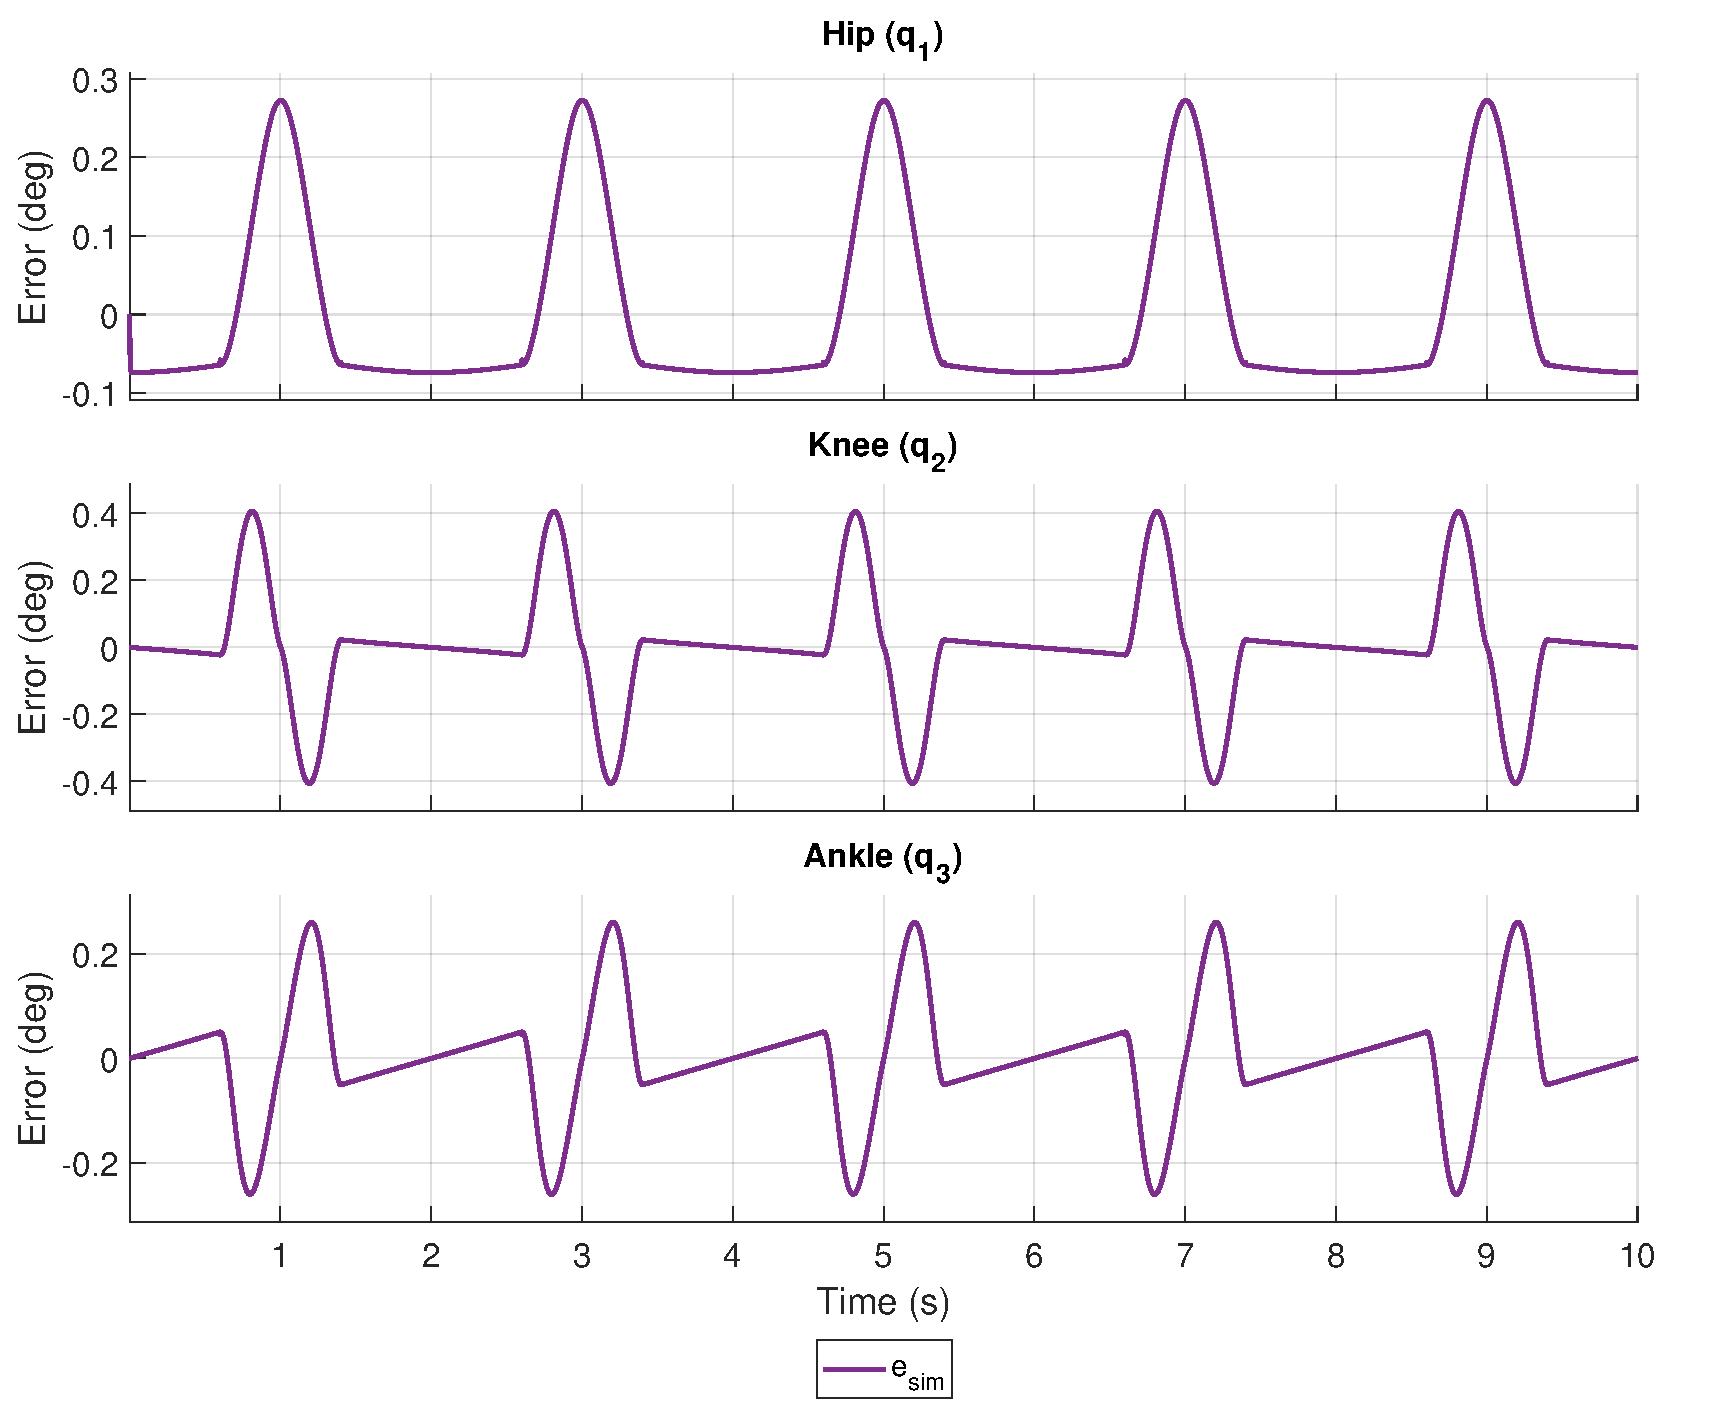
\includegraphics[width=\textwidth]{images/joint_errors.pdf}
        \caption{Tracking Errors}
    \end{subfigure}
    \caption{Joint-Space Simulation Results.}
    \label{fig:joint_results}
\end{figure}
